% Weak convergence: two bumps sliding onto a point mass.
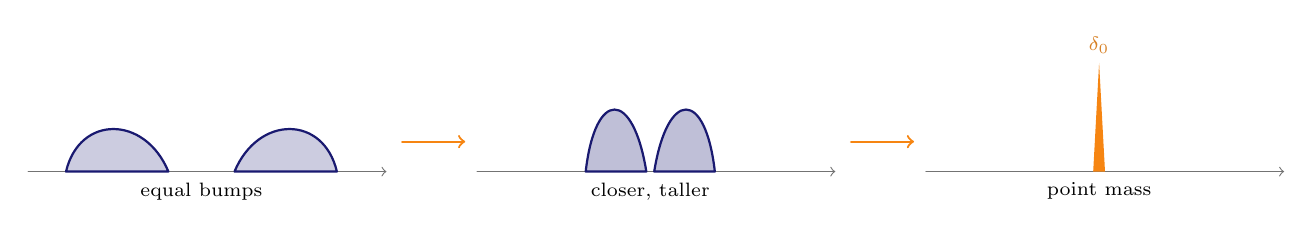
\begin{tikzpicture}[x=1cm,y=1cm,line join=round,line cap=round]
  \draw[black!55,->] (-2.2,0) -- (2.35,0);
  \draw[MidnightBlue,thick,fill=MidnightBlue!22]
    (-1.72,0) .. controls (-1.55,0.72) and (-0.72,0.72) .. (-0.42,0) -- cycle;
  \draw[MidnightBlue,thick,fill=MidnightBlue!22]
    (0.42,0) .. controls (0.72,0.72) and (1.55,0.72) .. (1.72,0) -- cycle;
  \node[font=\scriptsize,below] at (0,-0.02) {equal bumps};

  \draw[BurntOrange,thick,->] (2.55,0.38) -- (3.35,0.38);

  \begin{scope}[xshift=5.7cm]
    \draw[black!55,->] (-2.2,0) -- (2.35,0);
    \draw[MidnightBlue,thick,fill=MidnightBlue!28]
      (-0.82,0) .. controls (-0.7,1.05) and (-0.22,1.05) .. (-0.05,0) -- cycle;
    \draw[MidnightBlue,thick,fill=MidnightBlue!28]
      (0.05,0) .. controls (0.22,1.05) and (0.7,1.05) .. (0.82,0) -- cycle;
    \node[font=\scriptsize,below] at (0,-0.02) {closer, taller};
  \end{scope}

  \draw[BurntOrange,thick,->] (8.25,0.38) -- (9.05,0.38);

  \begin{scope}[xshift=11.4cm]
    \draw[black!55,->] (-2.2,0) -- (2.35,0);
    \fill[BurntOrange] (-0.075,0) -- (0,1.38) -- (0.075,0) -- cycle;
    \node[font=\scriptsize,BurntOrange!85!black,above] at (0,1.38) {$\delta_0$};
    \node[font=\scriptsize,below] at (0,-0.02) {point mass};
  \end{scope}
\end{tikzpicture}
